%%%%%%%%%%%%%%%%%%%%%%%%%%%%%%%%%%%%%%%%%%%%%%%%%%%%%%%%%%%%%%%%%%%%%%%%%%%%%%%%%%%%%%%%%%%%%%%%
%
% CS484 Written Question Template
%
% Acknowledgements:
% The original code is written by Prof. James Tompkin (james_tompkin@brown.edu).
% The second version is revised by Prof. Min H. Kim (minhkim@kaist.ac.kr).
%
% This is a LaTeX document. LaTeX is a markup language for producing 
% documents. Your task is to fill out this document, then to compile 
% it into a PDF document. 
%
% 
% TO COMPILE:
% > pdflatex thisfile.tex
%
% If you do not have LaTeX and need a LaTeX distribution:
% - Personal laptops (all common OS): www.latex-project.org/get/
% - We recommend latex compiler miktex (https://miktex.org/) for windows,
%   macTex (http://www.tug.org/mactex/) for macOS users.
%   And TeXstudio(http://www.texstudio.org/) for latex editor.
%   You should install both compiler and editor for editing latex.
%   The another option is Overleaf (https://www.overleaf.com/) which is 
%   an online latex editor.
%
% If you need help with LaTeX, please come to office hours. 
% Or, there is plenty of help online:
% https://en.wikibooks.org/wiki/LaTeX
%
% Good luck!
% Min and the CS484 staff
%
%%%%%%%%%%%%%%%%%%%%%%%%%%%%%%%%%%%%%%%%%%%%%%%%%%%%%%%%%%%%%%%%%%%%%%%%%%%%%%%%%%%%%%%%%%%%%%%%
%
% How to include two graphics on the same line:
% 
% \includegraphics[width=0.49\linewidth]{yourgraphic1.png}
% \includegraphics[width=0.49\linewidth]{yourgraphic2.png}
%
% How to include equations:
%
% \begin{equation}
% y = mx+c
% \end{equation}
% 
%%%%%%%%%%%%%%%%%%%%%%%%%%%%%%%%%%%%%%%%%%%%%%%%%%%%%%%%%%%%%%%%%%%%%%%%%%%%%%%%%%%%%%%%%%%%%%%%

\documentclass[11pt]{article}

\usepackage[english]{babel}
\usepackage[utf8]{inputenc}
\usepackage[colorlinks = true,
linkcolor = blue,
urlcolor  = blue]{hyperref}
\usepackage[a4paper,margin=1.5in]{geometry}
\usepackage{stackengine,graphicx}
\usepackage{fancyhdr}
\setlength{\headheight}{15pt}
\usepackage{microtype}
\usepackage{times}

% From https://ctan.org/pkg/matlab-prettifier
\usepackage[numbered,framed]{matlab-prettifier}

\frenchspacing
\setlength{\parindent}{0cm} % Default is 15pt.
\setlength{\parskip}{0.3cm plus1mm minus1mm}

\pagestyle{fancy}
\fancyhf{}
\lhead{Homework 2 Questions}
\rhead{CS484}
\rfoot{\thepage}

\date{}

\title{\vspace{-1cm}Homework 2 Questions}


\begin{document}
	\maketitle
	\vspace{-3cm}
	\thispagestyle{fancy}
	
	\section*{Instructions}
	\begin{itemize}
		\item 4 questions.
		\item Write code where appropriate.
		\item Feel free to include images or equations.
		\item Please make this document anonymous.
		\item \textbf{Please use only the space provided and keep the page breaks.} Please do not make new pages, nor remove pages. The document is a template to help grading.
		\item If you really need extra space, please use new pages at the end of the document and refer us to it in your answers.
	\end{itemize}

	\section*{Questions}
	
	\paragraph{Q1:} Explicitly describe image convolution: the input, the transformation, and the output. Why is it useful for computer vision?
	
	%%%%%%%%%%%%%%%%%%%%%%%%%%%%%%%%%%%
	\paragraph{A1:} 
	When you have the image matrix I[width,height] and filter f[width,height],
	the convolution matrix h is following 
	
	\[h[m,n] = \sum_{k,l}^{} f[k,l] I[m-k,n-l]]

	\emph{We can get the response by going through the filter over the image. 
	For example, we can extract the horizontal edge of the image by 
	calcualting the convolution of the image and [1 0 1] filter.}
	
	
	%%%%%%%%%%%%%%%%%%%%%%%%%%%%%%%%%%%
	
	% Please leave the pagebreak
	\pagebreak
	\paragraph{Q2:} What is the difference between convolution and correlation? Construct a scenario which produces a different output between both operations.
	
	\emph{Please use \href{https://www.mathworks.com/help/images/ref/imfilter.html}{$imfilter$} to experiment! Look at the `options' parameter in MATLAB Help to learn how to switch the underlying operation from correlation to convolution.}
	
	%%%%%%%%%%%%%%%%%%%%%%%%%%%%%%%%%%%
	\paragraph{A2:} 

	\emph{Correlation shows the similarity of two data. Therefore, we can 
	calculate the similarity of two images by calculating the correlation of them after
	normalize. (Cosign similarity is one of the method) When you use this on two same image, 
	the normalized correlation value is maximized when two images are exactly overlapped.}

	\emph{On the other hand, convolution is the multicative response when the data 
	go through the signal. For example, when the image go through the low pass filter, 
	the high frequency component dissapear.}


	
	
	
	%%%%%%%%%%%%%%%%%%%%%%%%%%%%%%%%%%%
	
	% Please leave the pagebreak
	\pagebreak
	\paragraph{Q3:} What is the difference between a high pass filter and a low pass filter in how they are constructed, and what they do to the image? Please provide example kernels and output images.
	
	%%%%%%%%%%%%%%%%%%%%%%%%%%%%%%%%%%%
	\paragraph{A3:} Your answer here.
	\emph{In case of the low pass filter, it has a tendency to average the wide area. Thus, 
	the image which is passed the low pass filter is robust on the pixel level difference and gets 
	smoother. On the other hand, in case of the high pass filter, it detect the stiff cliff of 
	the pixel value. Therefore, it has a large value when some pixel's value drastically changed 
	compare to the neighbor pixel. Following is the example of the LPF and HPF.}
	\[
		LPF =
	   \left[ {\begin{array}{ccc}
		\frac{1}_{9} & \frac{1}_{9} & \frac{1}_{9} \\
		\frac{1}_{9} & \frac{1}_{9} & \frac{1}_{9} \\
		\frac{1}_{9} & \frac{1}_{9} & \frac{1}_{9} \\
	   \end{array} } \right]      HPF = 
	   \left[ {\begin{array}{ccc}
		0 & -\frac{1}_{2} & 0 \\
		-\frac{1}_{2} & 2 & -\frac{1}_{2} \\
		0 & -\frac{1}_{2} & 0 \\
	   \end{array} } \right]
	 \]
	
	\emph{Following is the example of the iamges which passed the low pass filter and high pass filter.}
	
	\begin{figure}[h]
		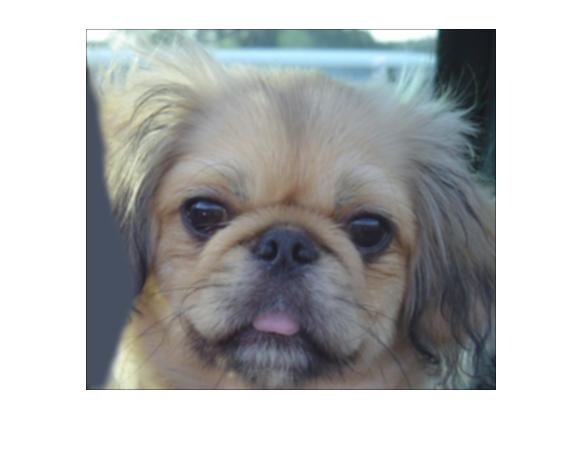
\includegraphics[width=6cm]{../lpimage.jpg}
		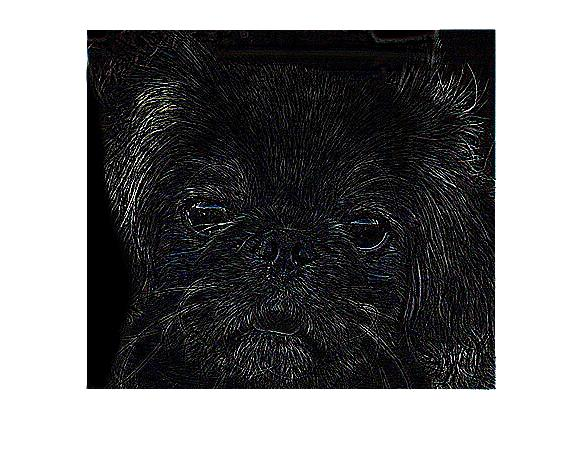
\includegraphics[width=6cm]{../hpimage.jpg}
		\caption{Left is LPF image and right one passed HPF }
		\label{fig:HPF}
	 \end{figure}

	\emph{LPF image got blurred and HPF image shows the edges}
	%%%%%%%%%%%%%%%%%%%%%%%%%%%%%%%%%%%
	
	% Please leave the pagebreak
	\pagebreak
	\paragraph{Q4:} How does computation time vary with filter sizes from $3\times3$ to $15\times15$ (for all odd and square sizes), and with image sizes from 0.25~MPix to 8~MPix (choose your own intervals)? Measure both using \href{https://www.mathworks.com/help/images/ref/imfilter.html}{$imfilter$} to produce a matrix of values. Use the \href{https://www.mathworks.com/help/images/ref/imresize.html}{$imresize$} function to vary the size of an image. Use an appropriate charting function to plot your matrix of results, such as \href{https://www.mathworks.com/help/matlab/ref/scatter3.html}{$scatter3$} or \href{https://www.mathworks.com/help/matlab/ref/surf.html}{$surf$}.
	
	Do the results match your expectation given the number of multiply and add operations in convolution?
	
	See RISDance.jpg in the attached file.
	
	%%%%%%%%%%%%%%%%%%%%%%%%%%%%%%%%%%%
	\paragraph{A4:} 
	\emph{Let's assume that there is a special operation for the matirx multiplication so the 
	computation time does not follow the linear proportion of the number of 
	element of thematrix. If the assumtion is true, then the computation time for
	8x8 filter and 15x15 filter will have linear or constant difference.
	However, as far as it requires same number of computation with the image size, (or larger matrix)
	the time for computation with 8Mpixel image will take almost 32times of 0.25Mpixel image's one.}
	
	\emph{Following is the experiment result. 1000times repeated and calcultated the average of the time.}
	 
	\emph{0.25M pixcel, 8x8 filter, 0.004084sec/img}
	 
	\emph{0.25M pixcel, 15x15 filter, 0.006916sec/img}
	 
	\emph{8M pixcel, 8x8 filter, 0.107183sec/img}
	 
	\emph{8M pixcel, 15x15 filter, 0.112047sec/img}

	\emph{16M pixcel, 15x15 filter, 0.232047sec/img}

	\emph{the time difference between 8x8 filter and 15x15 filter does not follow the linear proportion, and the difference between 0.25M image and 8M image 16M image roughly follow the linear proportion. }
	
	%%%%%%%%%%%%%%%%%%%%%%%%%%%%%%%%%%%
	
	
	% If you really need extra space, uncomment here and use extra pages after the last question.
	% Please refer here in your original answer. Thanks!
	%\pagebreak
	%\paragraph{AX.X Continued:} Your answer continued here.
	
	
	
\end{document}